%\section{Improved Architecture\\Incorporating into Bridges\\Protecting Bridges}
\section{Protecting Bridges}
\label{sec:active-protect}

Sections~\ref{sec:retro-results} and~\ref{sec:live-audit} showed how
applying the balance invariant can identify attacks retrospectively and
monitor ongoing transactions as an external third party without any
changes to existing bridge infrastructure.  However, the live
monitoring system only alerts on violations of the invariant and does
not prevent violating bridge transactions from being processed.

In this section, I describe an approach for extending an existing
bridge implementation to prevent malicious transactions from
executing.  Our goal is to present a proof-of-concept implementation
to demonstrate the feasibility of applying the balance invariant in the
workflow of bridge transactions as an active defense against malicious
transactions.  We acknowledge that several practical issues remain
for a complete operational system, presenting an opportunity for
interesting future work.

%% explore the question of whether it is possible to implement a
%% mechanism that stops malicious transactions from execution with
%% minimal code changes.

% how hard it would be to modify the Wormhole bridge to prevent transactions that violate the invariant from being processed. We propose an improved architecture that treats the bridge relaying infrastructure as a black box and can effective stop any malicious transactions that break the invariant and caused by code bugs.

% Below, I start by answering the question of where to introduce the mechanism. Then, using Wormhole as an example, I show how I can modify the bridge to prevent malicious transactions from being processed with fewer than 30 lines of code changes. Finally, I evaluate the security and performance of the improved architecture.

We start by proposing a new model for the workflow of bridge
transactions.  Then, using Wormhole as an example, I show how to
modify an existing bridge implementation to prevent malicious transactions from
being processed with fewer than 30 lines of code changes.  Finally, we
evaluate the correctness and overhead of this initial implementation.

\subsection{The Announce-then-Execute Model}

To guide the design of a new model, I first highlight where the
attack surfaces exist. As shown in Figure~\ref{fig:cross-chain}, a
vulnerability can exist in as early as the second step (verify lock
amount) to as late as the next-to-last step (verify relayed
transaction). Thus, a natural place to introduce a protection
mechanism is just before the final step, which executes the relayed
transaction.

Using this insight I propose an announce-then-execute model.
Figure~\ref{fig:improved-arch} depicts the entities and steps involved
in the new model, focusing on the destination chain (replacing the
right-most box of Figure~\ref{fig:cross-chain}).  The new model
employs two steps to process a withdrawal transaction: (1) verify and
announce the withdrawal transaction on the destination blockchain (steps
8 and 9) and (2) execute the withdrawal transaction (steps 11 and
12). Of particular note, this new model introduces an additional
entity, the \emph{Approver}, which is responsible for approving the
relayed transaction before it is executed.  The Approver can be a bridge
operator, a trusted or trustless third-party (e.g., Bascule~\cite{bascule},
inspired by our work, uses trusted execution environments instead of consensus to ensure the safety of the approver), or a set of
third-parties (e.g., using
multisig for decentralized control). It is responsible for
verifying that the announced withdrawal transaction satisfies the
invariant by validating the same conditions as the Auditor in the live
monitoring system (Section~\ref{sec:live-audit}).  If the relayed
transaction violates the invariant, the Approver can reject the
transaction to prevent it from being executed.

% In addition, I observe that many bridges (e.g., Wormhole) couple the last two steps tightly --- the verification and execution of the relayed transaction are done in the same function call. While being gas efficient, this implementation has a critical drawback. Namely, if the verification function has a bug, it would be impossible to stop the malicious transaction from being executed.

% This means that the verification of a relayed transaction is done at the same time as the execution of the relayed transaction. 

\begin{figure}[t]
\centering
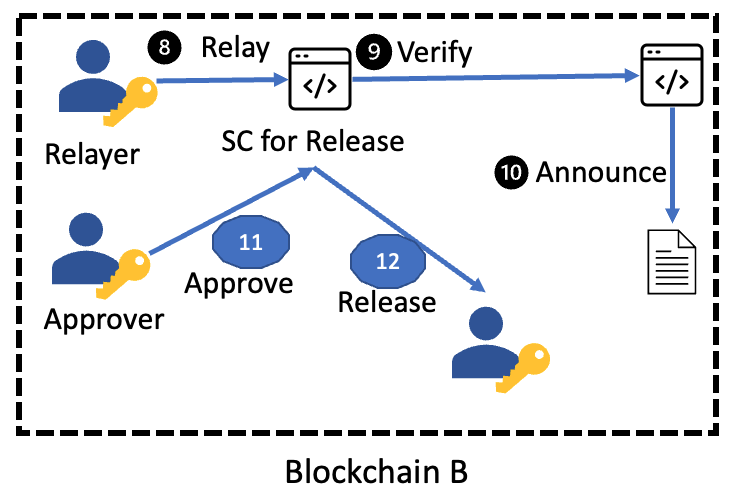
\includegraphics[width=0.9\columnwidth]{fig/improved.pdf}
\caption[Announce-then-Execute Model for Bridges]{Announce-then-execute model for bridges. The approver verifies the relayed transaction before its execution. The approver can be implemented differently (e.g., a set of third-parties), depending on the desired security properties.}
\label{fig:improved-arch}
% \vspace{-0.1in}
\end{figure}


\subsection{Threat Model, Assumptions, and Trade-offs}
We assume that the approver is able to independently verify the relayed transaction and the correct amount of tokens to be transferred. Under this assumption, the announce-then-execute model prevents any implementation bug in any existing bridge components, from step 2 (e.g., the bridge fails to compute the correct deposit amount) to step 8 (e.g., the bridge fails to verify the signature of a relayed transaction). Further, if the 
approver uses secure hardware (namely, HSMs) or a decentralized third-parties
(e.g., with multisig), the model can provide additional protection against
insider threats and key theft (e.g., up to the multisig threshold). Of course,
if the bridge is the only approver, the model does not provide any additional
protection against such insider threats or key theft attacks.


The announce-then-execute model has a few advantages. First, it
explicitly separates the verification and execution of the relayed
transaction, thereby providing an opportunity to reject transactions
that violate the balance invariant.  In comparison, many bridges (e.g.,
Wormhole) couple the last two steps tightly --- the same function call
performs both the verification and execution of the relayed
transaction.  As a result, if the verification step has a bug, it is
not possible to stop violating transactions from being
executed.

Second, the announce-then-execute model allows any external
party, that has visibility into both blockchains, to determine if the
relayed transaction violates the invariant. A long-standing challenge
with bridges is the oracle problem: the destination blockchain does
not have visibility into the source blockchain. The
announce-then-execute model side-steps the oracle problem by allowing
an external party to verify the relayed transaction before it is
executed. This external party can be the bridge operator or a group of third-parties.
Moreover, the announce-then-execute model is compatible with
existing bridges, as it only requires modification to the last step
and treats the relaying infrastructure as well as the verification
code as a black box. In fact, Wormhole's implementation on Solana already separates the process of verifying and executing the relayed transaction, making it even easier to adopt the announce-then-execute model. Had they implemented the announce-then-execute model, the Wormhole bridge would have been able to prevent the \$360M attack on the Solana network~\cite{wormholeattack}.

Lastly, the announce-then-execute model does not
introduce any new attack surfaces --- even if the approver naively
approves all transactions, an attacker still has to exploit other
vulnerabilities in the bridge to profit.

\subsection{Implementation}

%% We took open-sourced Wormhole code written in solidity and modified it to implement the announce-then-execute mechanism.
%% Wormhole's current withdraw function performs two tasks:
%% it verifies the signatures that authorize the withdraw transaction and then executes the withdraw transaction. We split the withdraw function into two separate functions: \texttt{announceWithdraw} and \texttt{approveWithdraw}. The \texttt{announceWithdraw} function handles signature verification and announces the withdraw transaction on the destination blockchain, while the \texttt{approveWithdraw} function executes the withdraw transaction. This modification required fewer than 30 lines of code changes.

Continuing our focus on Wormhole from Section~\ref{sec:live-audit}, we
modified one of Wormhole's open-source contracts to implement the
announce-then-execute model.  Wormhole's current withdrawal function
performs two tasks: it verifies the signatures that authorize the
withdrawal transaction, and then executes it. We
split the withdrawal function into two separate functions:
\texttt{announceWithdraw} and \texttt{approveWithdraw}. The
\texttt{announceWithdraw} function handles signature verification and
announces the withdrawal transaction,
while the \texttt{approveWithdraw} function executes the withdrawal
transaction. This modification required fewer than 30 lines of code
changes.

For simplicity, I opted for a single approver with one key in our implementation. However, our implementation can be easily extended (e.g., to use multisig). In addition, while our implementation has not been adopted by the Wormhole team (as I are a research group not affiliated with Wormhole), our solution has inspired other industry projects to adopt a similar approach~\cite{bascule}.

\subsection{Evaluation}

As a final step I performed a high-level evaluation of the
correctness and overhead (in terms of gas usage) of the
announce-then-execute implementation.  We deployed our bridge
implementation on the Binance and Fantom testnets due to the
availability of free faucets for acquiring testnet tokens for them.
We then executed a series of benign and malicious transactions using
Binance as the source chain and Fantom as the destination chain.

% , and tracked their gas usage during execution.

%% (would be fine if this were a long eval, but since it's so short it's
%% not really needed)
%%
%% We demonstrate that the improved architecture
%% can effectively stop all three malicious transactions while allowing
%% benign transactions to proceed. We also show that the overhead of the
%% improved architecture incurs only a moderate overhead of 50\% more gas
%% usage without any optimization.

\textbf{Correctness.}  For evaluating correctness I disabled the
security checks in the original implementation (e.g., signature
verification) to allow malicious transactions to flow through the
contract implementation (e.g., simulating key compromise).  We then
executed 100 pairs of deposit and withdrawal transactions to validate
that the implementation correctly identifies and protects itself
against malicious transactions that violate the balance invariant.

All but three of the 100 paired transactions were benign, and used
randomly generated values as transaction inputs.
%
The remaining three paired transactions were malicious and were
randomly placed in the transaction sequence.  The malicious
transactions represented the three kinds of bugs underlying the
large attacks in Section~\ref{sec:retro-results}: (1) a bug that
allows a user to withdraw more tokens than they deposited, (2) a bug
that allows a user to withdraw tokens without depositing any
(simulating key compromise), and (3) a bug that allows a user to
withdraw twice from the same deposit (double spending).

The bridge implementation correctly executed the benign transactions
to completion and rejected the three malicious transactions.  The
results are the same independent of where the malicious transactions
randomly appear in the sequence.

\textbf{Overhead.}  The additional steps add overhead to implementing
bridges.  For this experiment, I measured the gas usage for executing
Wormhole's original implementation (with its security checks) and the
gas usage of the announce-then-execute implementation (also with the
original security checks plus our added code).  On average, our
proof-of-concept implementation consumed 110\thou more gas than the
original implementation (370\thou vs.\ 260\thou gas) when
executing the benign transactions, which translates to a
roughly \$1 increase for a typical withdrawal on Ethereum.
% a 50\% increase in gas usage.

We note that our implementation is not optimized for gas usage, and
these results indicate that an
% real
operational deployment
% of the announce-then-execute model
will likely want to reduce the gas overhead of
the additional work (e.g., narrowing to transactions above a threshold
amount of funds).  As discussed further in Section~\ref{sec:discuss},
such optimizations and other practical issues of a real deployment are
interesting future work.

